\chapter{Delay Differential Equations}\label{sec:delay-differential-equations}

\section{Piecewise Continuous Functions}
    \label{sec:piecewise-continuous-functions}
    
    The following definition is motivated by capturing the character evolution arising from hybrid systems. We will see that we can consider such to be piecewise continuous.

    % \begin{definition}[Piecewise Continuous]\label{def:piecewise-continuous}
    %     Let $D=[a,b]\subseteq\R$ be a closed interval (this includes the cases when $a=-\infty$ or $b=\infty$, or both). The mapping $x:D\rightarrow\R^n$ is called \emph{piecewise continuous} if and only if there is a finite subdivision $\{t_i:i=\range{0}{m}\}$ of $D$ (i.e.\ $a=t_0<t_1<\ldots<t_m=b$) such that $x$ is continuous on each interval piece $[t_i,t_{i+1})$ for all $i=\range{0}{m-1}$ and the left sided limits
    %     \begin{equation}
    %         \lim_{\substack{t\upto t_{i+1}\\ t\in[t_i,t_{i+1})}} x(t)
    %     \end{equation}
    %     exist. Hence $x(b)$ can be an isolated point and this right interval limit $b$ is the only spot where such is allowed.

    %     We denote by $\Cnpw[0]{D}{\R^n}$ the set of \emph{piecewise continuous functions} on the compact interval $D$ (this excludes the cases with $\pm\infty$), mapping to $\R^n$.
    % \end{definition}

    \begin{definition}[Piecewise Continuously Differentiable]\label{def:pw-cont-diff}
        Let $D=[a,b]\subseteq\R$ be a closed interval (this includes the cases when $a=-\infty$ or $b=\infty$, or both). The mapping $x:D\rightarrow\R^n$ is called $n$-times \emph{piecewise continuously differentiable} if and only if there is a finite subdivision $\{t_i:i=\range{0}{m}\}$ of $D$ (i.e.\ $a=t_0<t_1<\ldots<t_m=b$) such that $x$ is $n$-times continuously differentiable on each interval piece $(t_i,t_{i+1})$ with continuable derivatives on $\compactum{t_i}{t_{i+1}}$.

        This means, for all $i=\range{0}{m-1}$ and for all $k=\range{0}{n}$ exist the left sided limits
        \begin{equation}
            \lim_{\substack{t\upto t_{i+1}\\ t\in(t_i,t_{i+1})}} \D[k]{x}(t)
        \end{equation}
        as well as the right sided limits
        \begin{equation}
            \lim_{\substack{t\downto t_{i}\\ t\in(t_i,t_{i+1})}} \D[k]{x}(t) = \D[k]{x}(t_i)
        \end{equation}
        which are supposed to coincide with the value of $\D[k]{x}$ at $t_i$.
        Hence $x(b)$ can be an isolated point and this right interval limit $b$ is the only spot where such is allowed.
        In the case $n=0$, we say $x$ is \emph{piecewise continuous}.

        We denote by $\Cnpw[n]{D}{\R^n}$ the set of \emph{$n$-times piecewise continuously differentiable functions} on the compact interval $D$ (this excludes the cases with $\pm\infty$), mapping to $\R^n$, and respectively, by $\Cnpw[0]{D}{\R^n}$ the \emph{piecewise continuous functions}.
    \end{definition}

    % TODO: sup-norm for pw

    \begin{lemma}[]\label{lm:pc-integrable}
        A \emph{piecewise continuous function}, as defined in Definition~\ref{def:pw-cont-diff} is (Riemann) integrable.
    \end{lemma}
    \begin{proof}
        See standard analysis literature, such as \cite{Rudin76PrinciplesAnalysis} or \cite{Gathmann12GDM}.
        % ObdA: one subint with jump at end
    \end{proof}

    The following lemma generalizes the fundamental theorem of calculus to piecewise continuous derivatives.

    \begin{lemma}[]\label{lm:pc-hauptsatz}
        Let $F\in\Cn[0]{\compactum{a}{b}}{}\cap\Cnpw[1]{\compactum{a}{b}}{}$ on the subdivision $\set{\range{t_0=a}{t_m=b}}$ of $\compactum{a}{b}\subset\R$.
        For all $s\in\compactum{a}{b}$ it holds
        \begin{equation*}
            F(s)-F(a) = \sum_{i=0}^k\int_{t_i}^{t_{i+1}}f(t)\dx[t] + \int_{t_k}^s f(t)\dx[t]
        \end{equation*}
        where $t_k\leq s < t_{k+1}$.
        % FIXME: what about a=-inf or b=inf?
    \end{lemma}
    \begin{proof}
        On each interval $\compactum{t_i}{t_{i+1}}$ of the subdivision, $F$ is continuously differentiable. Hence, by the the fundamental theorem of calculus (cf. standard analysis literature, e.g. \cite{Gathmann12GDM,Rudin76PrinciplesAnalysis}) it follows for all $i=\range{0}{m-1}$:
        \begin{equation*}
            F(t_{i+1})-F(t_i) = \int_{t_i}^{t_{i+1}}\D{F}(t)\dx[t]
        \end{equation*}
        and
        \begin{equation*}
            F(s)-F(t_k) = \int_{t_k}^{s}\D{F}(t)\dx[t]
        \end{equation*}
        % TODO: by continuity, F(t_i)=F(t_i)
        Summation over $i=\range{0}{k}$ gives the ... as a telescope sum (since $F$ continuous on $\compactum{a}{b}$)
        \begin{equation*}
            F(s)-F(a) = \sum_{i=0}^k\int_{t_i}^{t_{i+1}}f(t)\dx[t] + \int_{t_k}^s f(t)\dx[t]
        \end{equation*}
    \end{proof}

% \begin{figure*}[h]\centering
%     \begin{subfigure}[t]{0.5\textwidth}\centering
%         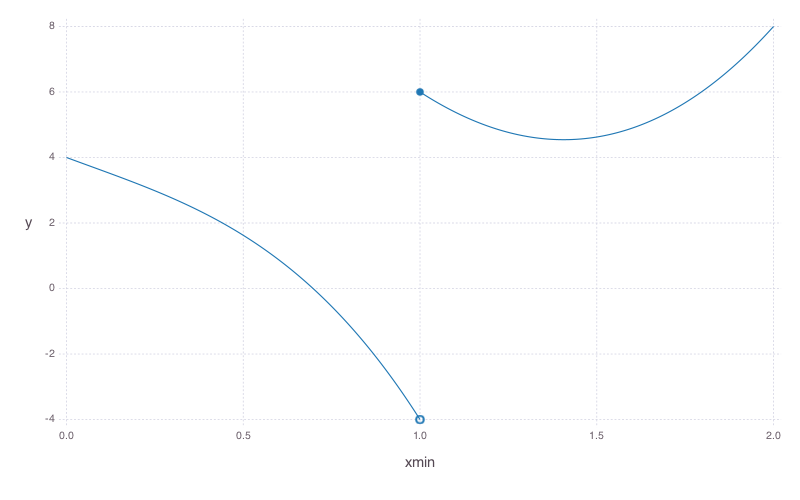
\includegraphics[width=\textwidth]{figures/allowed.png}
%         \caption{Admissible piecewise continuous function.}
%         \label{fig:allowed}
%     \end{subfigure}
%     \begin{subfigure}[t]{0.5\textwidth}\centering
%         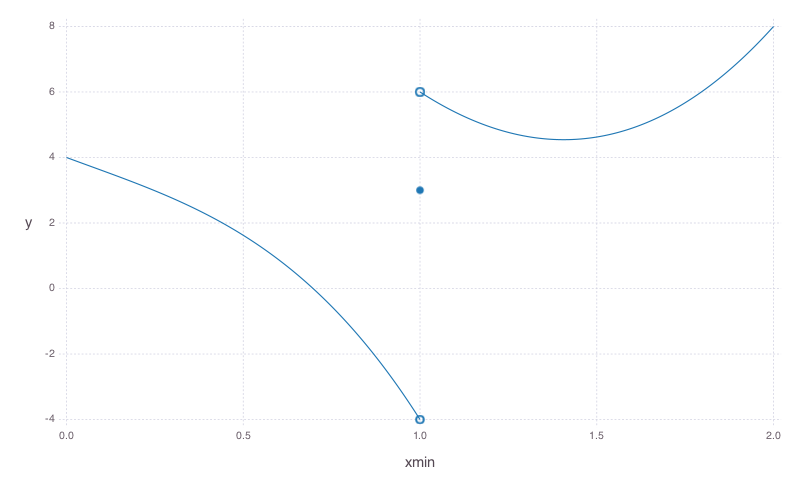
\includegraphics[width=\textwidth]{figures/not-allowed.png}
% 	    \caption{Not allowed!}
% 	    \label{fig:not-allowed}
%     \end{subfigure}
%     \caption{Examples to Definition \ref{definition-piecewise-continuous}.}
% \end{figure*}


\section{Definition DDE}
    \label{sec:definition-dde}

    \begin{definition}[Delay Differential Equation]\label{def:dde}
        Let $f\from\deff\to\R^n$ and $\tau > 0$.
        A functional equation of the form
        \begin{equation}\label{eq:dde}
            \D{x}(t) = f(t,x(t),x(t-\tau))
        \end{equation}
        is called \emph{Delay Differential Equation (DDE)} with \emph{constant, discrete delay $\tau$}.
        It is \emph{autonomous} if its right hand side $f$ is time independent and \emph{pure} if the right hand side only depends on $x(t-\tau)$ and not on $x(t)$.

        A DDE can be equipped with an \emph{initial condition} $x_{\tzero}$. It specifies the values of $x$ on $[\tzero-\tau, \tzero]$ on which the right hand side depends.
        Such a pair is called \emph{initial value problem (IVP)}:
        \begin{equation}\label{eq:ivp}
            \begin{cases}
                \D{x}(t) = f(t,x(t),x(t-\tau)) & \text{for } t\geq\tzero\\
                x(t) = x_{\tzero}(t) & \text{for } t\in [\tzero-\tau,\tzero]
            \end{cases}
        \end{equation}
    \end{definition}

    % Since we only consider autonomous DDEs, we can without loss of generality restrict to the case of initial time $t_0=0$.

    The definition of a DDE can be extended to multiple constant discrete delays. For simplicity, we restrict here to a single delay.


\section{Definition of Solution}
    \label{sec:definition-of-solution}

    \begin{definition}[Solution of DDE]\label{def:solution-dde}
        A function $x\from\compactum{\tzero-\tau}{\tzero+T}\to\R^n$ is called \emph{(local) solution} of the initial value problem~\eqref{eq:ivp}, if and only if
        %there exists a $T>0$ such that
        $\restrict{x}{(\tzero,\tzero+T)}\in \Cn[1]{(\tzero,\tzero+T)}{\R^n}$ with
        \begin{equation*}
            \D{x}(t) = f(t,x(t),x(t-\tau))
        \end{equation*}
        for all $t\in (\tzero,\tzero+T)$ and in $t=\tzero$, it holds for the right-hand derivative
        \begin{equation*}
            \lim_{h\downto \tzero}\frac{x(h)-x(\tzero)}{h}=f(\tzero,x(\tzero),x(\tzero-\tau))
        \end{equation*}
        and obeys the initial condition:
        \begin{equation*}
            x(t) = x_{\tzero}(t) \quad\text{for } t\in [\tzero-\tau,\tzero].
        \end{equation*}
        If the function $x$ is a solution for all $T>0$, it is called \emph{global}.

        %TODO: differentiable in right rand point? need not derivative in right hand point
        %TODO: Fortsetzbarkeit For example initial condition has jump, this point is limit for local solution.
    \end{definition}

% \begin{figure}[h]\centering
%     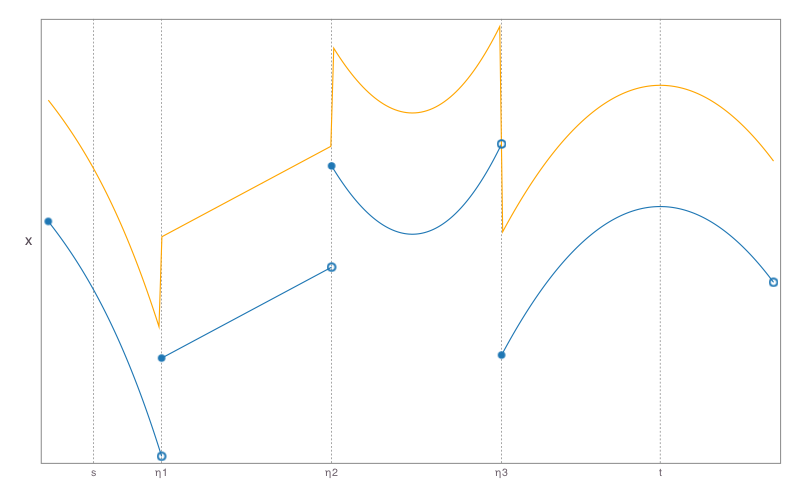
\includegraphics[width=\textwidth]{figures/multiple.png}
% 	\caption{Illustration of proof to Lemma \ref{lemma-continuity}}
% 	\label{fig:not-allowed}
% \end{figure}

% FIXME: This lemma is wrong. Show instead integrability of f(t,x_t)
\begin{lemma}
    \label{lemma-continuity}

    % Let $x:[\tzero-\tau,\tzero+T] \rightarrow \R^n$ be piecewise continuous (as in Definition \ref{definition-piecewise-continuous}) with the subdivision $\{t_0,\ldots,t_k\}$, i.e. there are $k$ subintervals.
    %
    % Then $t \mapsto x_t = x(t+\theta)$, where $\theta\in[-\tau,0]$, is a piecewise continuous mapping from $[\tzero,\tzero+T]$ into $\statespace[\tau]$.
\end{lemma}

\begin{proof}
    % $x$ is piecewise continuous and hence uniformly piecewise continuous on the compact interval $I=[\tzero-\tau,\tzero+T]$.
    % i.e. uniformely continuous on each subinterval with stetiger Fortsetzung in right side.
    % \begin{equation}
    %     \forall\epsilon >0 \exists\delta_i >0 \forall t,s\in I_i: \quad \abs{t-s}<\delta_i \Rightarrow \nnorm{x(t)-x(s)}<\epsilon
    % \end{equation}
    % Let $\epsilon > 0$. $x|_{[t_i,t_{i+1}]}$ (with stetiger fortsetzung in right interval limit) is uniformly continuous, i.e. there is a $\delta_i > 0$ (for the given $\epsilon$), such that $\forall\,t, s \in [t_i,t_{i+1}]$ holds
    % % TODO: can use \leq ?
    % \begin{equation}
    %     \abs{t-s} < \delta_i \Rightarrow \nnorm{x(t)-x(s)} < \epsilon
    % \end{equation}
    %
    % Among the given $\delta_i$, choose the smallest as $\delta = \min_i \delta_i$.
    %
    % For any $i$ and $s,t\in [t_i,t_{i+1})\subset [\tzero,\tzero+T]$ with $\abs{t-s}<\delta$, it holds
    % \begin{equation}
    %     \supnorm{x_t - x_s} = \sup_{\theta\in [-\tau,0]}\nnorm{x(t+\theta) - x(s+\theta)} < \epsilon
    % \end{equation}
    % since $t+\theta, s+\theta \in I$
    % Hence $t \mapsto x_t$ is uniformely continuous on $[t_i,t_{i+1})$.
\end{proof}


\section{Method of Steps}
    \label{sec:method-of-steps}
    
    for $t\in [0,\tau]$, $x$ must satisfy the following ordinary initial value problem obtained by plugging the initial function into equation (??). For suitable $f$ and $x_0$, the existence (and uniqueness) of a solution on $[0,\tau]$ is guaranteed by ODE theory (\ldots{} or Picard-Lindelöf theorems).

    This procedure can then be applied repeatedly to extend the obtained solution by steps of length $\tau$.





\section{Existence and Uniqueness of Solutions}
    \label{solutions-existence-uniqueness}

    will consider rhs cont and lip
    $f$ Lipschitz with piecewise continuous initial function have existence and uniqueness ???? smoothing

    \begin{definition}[Lipschitz Continuity]\label{def:lipschitz}
        % similar to \cite{pruesswilke10GewDiffGl,Smith10IntroDDE}
        A function $f\from\deff\to\R^n$ is called \emph{(locally) Lipschitz continuous} in its second argument if and only if for all $a,b\in\R$ and $M>0$ there is a $L>0$ such that
        \begin{equation}
            \nnorm{f(t,x,y) - f(t,\bar{x},y)} \leq L\nnorm{x - \bar{x}}
        \end{equation}
        for all $t\in [a,b]$ and $x,\bar{x},y\in\R^n$ with $\nnorm{x},\nnorm{\bar{x}},\nnorm{y}\leq M$.
    \end{definition}

    \begin{lemma}\label{lm:bounded-lipschitz}
        Let $f\from\deff\to\R^n$ be continuous and Lipschitz continuous in its second argument.

        For any given compact interval $\compactum{a}{b}$ and $M>0$ there exists a bound $K>0$ such that
        \begin{equation}
            \nnorm{f(t,x,y)}\leq K
        \end{equation}
        for all $t\in\compactum{a}{b}$ and $x,y\in\R^n$ with $\nnorm{x},\nnorm{y}\leq M$.
    \end{lemma}
    \begin{proof}
        Let $L$ be the Lipschitz constant of $f$ for the given $\compactum{a}{b}$ and $M$. Then
        \begin{multline*}
            \nnorm{f(t,x,y)} \leq \nnorm{f(t,x,y) - f(t,0,y)} + \nnorm{f(t,0,y)}\\
            \leq L\nnorm{x-0} + \nnorm{f(t,0,y)} \leq LM+P = K
        \end{multline*}
        for $t\in\compactum{a}{b}$ and $x,y\in\R^n$ with $\nnorm{x},\nnorm{y}\leq M$. We used the continuity of $f$ on the compact set $S=\compactum{a}{b}\times\set{z\in\R^n\with\nnorm{z}\leq M}$ for the existence of
        \begin{equation*}
            P = \max_{(s,z)\in S}\nnorm{f(s,0,z)}
        \end{equation*}
    \end{proof}

    \begin{lemma}\label{lm:integral-equation}
        %TODO: solving dde equiv to solving integral equation??? (-\textgreater{} Lemma) and compare with ODE lecture notes
        Finding a solution of the initial value problem~\eqref{eq:ivp} is equivalent to solving the integral equation
        integral componentwise, f vector valued
        \begin{equation}
            x(t) = x_{\tzero}(\tzero) + \int_{\tzero}^t f(s,x(s),x(s-\tau))\dx[s]
        \end{equation}
        and is continuous in t.
    \end{lemma}
    \begin{proof}
        integrate from discontinuity of $\xbartaut{t}$ to discontinuity and proof stetige fortsetzbarkeit at these points
    \end{proof}

    \begin{theorem}[Existence of unique solution]\label{thm:solution-existence}
        Consider the Delay Differential Equation
    %TODO: do we need global existence or just local?
        \begin{equation}
            \begin{cases}
                \D{x} = f(t,x(t),x(t-\tau)) & \text{for } t\geq\tzero\\
                x(t) = x_\tzero(t-\tzero)   & \text{for } t\in [\tzero-\tau,\tzero]
            \end{cases}
        \end{equation}
        with $f\from\deff\to\R^n$ continuous and satisfying the (local) Lipschitz condition in its second argument (Def.~\ref{def:lipschitz}).

        % where $\nnorm{\cdot}$ denotes the Euclidian norm on $\R^n$ and $\supnorm{\cdot}$ the supremum norm of the Banach space of continuous functions on $[-\tau,0]$.

        Then for each \emph{initial condition} $x_{\tzero}\in\statespace[\tau]$ and start time $\tzero$, there \textbf{exists} a \textbf{unique local solution} of the IVP on a time interval $[\tzero-\tau, \tzero+T]$. The duration $T>0$ depends on the sup-norm and discontinuity points of the initial condition. (?)
    \end{theorem}

    The proof is smiliar to the proof of the existence theorem (Theorem 3.7) given in~\cite{Smith10IntroDDE}.
    \begin{proof}
        As a piecewise continuous function, the initial condition can bounded by $M\geq \supnorm{x_\tzero}$ on $\delayinterval[\tau]$.
        
        If $\set{\range{-\tau=t_0}{t_k=0}}$ is the subdivision of $x_{\tzero}$, we choose $T=\min\set{t_0+\tau,\frac{M}{K}}$.
        
        % FIXME: M or 2M?
        Let $K>0$ be the upper bound for $f$ from Lemma~\ref{lm:bounded-lipschitz} on the set $S=[\tzero,\tzero+T] \times \{x\in R^n: \nnorm{x}\leq 2M\}\times \{y\in R^n: \nnorm{y}\leq 2M\}$ and $L>0$ the Lipschitz constant of $f$ for that set.

        % FIXME: why continuous? its pw cont?
        We construct a series $(x_{(m)})_{m\in\N_0}$ of continuous(?) functions which approximates the solution.
        Set
        \begin{equation}
            x_{(0)}(t)= \begin{cases}
                x_\tzero(0) & t\in [\tzero,\tzero+T]\\
                x_\tzero(t-\tzero) & t\in [\tzero-\tau,\tzero]
            \end{cases}
        \end{equation}
        For $m\in\N_{>0}$ define
        \begin{equation}
            x_{(m)}(t)= \begin{cases}
                x_\tzero(0) + \int_\tzero^t f(s,x_{(m-1)}(s),x_{(m-1)}(s-\tau))\dx[s] & t\in [\tzero,\tzero+T]\\
                x_\tzero(t-\tzero) & t\in [\tzero-\tau,\tzero]
            \end{cases}
        \end{equation}
        % FIXME: why exists integral?
        Integral exists
        It holds for all $m>0$ and $t\in \compactum{\tzero-\tau}{\tzero}$ by definition of the series
        \begin{equation}
            \nnorm*{x_{(m)}(t)-x_{(m-1)}(t)}=0
        \end{equation}
        We show by induction over $m$ that for all $t\in [\tzero,\tzero+T]$ it holds
        \begin{equation}
            \nnorm*{x_{(m)}(t)-x_{(m-1)}(t)} \leq \frac{K}{L}\frac{L^m (t-\tzero)^m}{m!}.
        \end{equation}
        Since obviously $\nnorm{x_{(0)}(t)}\leq M$, the statement for $m=0$ follows from the boundedness of $f$ on $S$ and the triangle inequality for integrals:
        \begin{equation}
            \nnorm{x_{(1)}(t)-x_{(0)}(t)} = \nnorm*{\int_\tzero^t f(s,x_{(0)}(s),x_{(0)}(s-\tau))\dx[s]} \leq K(t-\tzero)
        \end{equation}
        Since for any $m>0$, it holds by the triangle inequality
        % FIXME: why x(m)(t) smaller than 2M, such that K holds?
        \begin{align}
            \nnorm*{x_{(m)}} &\leq \nnorm*{x_\tzero(0)} + \int_\tzero^t \nnorm*{f(s,x_{(m)}(s),x_{(m)}(s-\tau))}\dx[s]\\
            &\leq M + K(t-\tzero) \leq M+KT\\
            &\leq 2M
        \end{align}
        In the inductive step we can apply the Lipschitz property of $f$
        \begin{multline*}
            \nnorm*{x_{(m+1)}(t)-x_{(m)}(t)}=\\
            = \nnorm*{\int_\tzero^t f(s,x_{(m)}(s),x_{(m)}(s-\tau)) - f(s,x_{(m-1)}(s),x_{(m-1)}(s-\tau))\dx[s]}\\
            \leq L \int_\tzero^t \nnorm*{x_{(m)}(s) - x_{(m-1)}(s)}\dx[s]\\
            \leq \frac{L^m K}{m!} \int_\tzero^t (s-\tzero)^m\dx[s]
            = \frac{L^m K}{(m+1)!}(t-\tzero)^{m+1}
        \end{multline*}
        We use this bound and the triangle inequality in
        \begin{multline*}
            \nnorm{x^{(m)}(t)-x^{(k)}(t)}\leq \nnorm*{x^{(m)}(t)-x^{(m-1)}(t)} + \nnorm*{x^{(m-1)}(t)-x^{(m-2)}(t)} +\ldots + \nnorm*{x^{(k+1)}(t)-x^{(k)}(t)}\\
            \leq \frac{K}{L}\frac{L^m (t-\tzero)^m}{m!} + \frac{K}{L}\frac{L^{m-1} (t-\tzero)^{m-1}}{(m-1)!} +\ldots +\frac{K}{L}\frac{L^{k+1} (t-\tzero)^{k+1}}{(k+1)!}\\
            \leq \frac{K}{L}\sum_{i=k+1}^\infty \frac{(LT)^i}{i!}
        \end{multline*}
        for any $k\in\N$ and $m\geq k$ and $t\in [\tzero,\tzero+T]$.
        This is the tail of the convergent exponential series and hence it converges to zero for $k\rightarrow\infty$.
        Since $x^{(m)}$ is continuous on $[\tzero,\tzero+T]$, this Cauchy sequence admits a limit $x$ in the Banach space $\continuouss[0]{[\tzero,\tzero+T]}{\R^n}$. Extend again to $[\tzero-\tau,\tzero]$ with $x_\tzero$, so $x\in\Cnpw[0]{[\tzero-\tau,\tzero]}{\R^n}$.


        Due to the uniform convergence of $x^(m)\rightarrow x$, we get uniform convergence of
        \begin{equation}
            f(s,x^{(m)}(s),x^{(m)}(s-\tau)) \rightarrow^{m\rightarrow\infty} f(s,x(s),x(s-\tau))
        \end{equation}
        and hence the integral and the limit process swap and by
        \begin{equation}
            x(t) = \lim_{m\rightarrow\infty} x^{(m+1)} = x_\tzero(0) + \lim_{m\rightarrow\infty}\int_\tzero^t f(s,x^{(m)}(s),x^{(m)}(s-\tau))\dx[s] = \int_\tzero^t f(s,x(s),x(s-\tau))\dx[s]
        \end{equation}
        it follows that $x$ solves the integral equation.
        This proofs the existence of a solution to the DDE. It remains to show uniqueness.

        % TODO: can one solution be on [\tzero, T_2] with T_2<T ?
        Let $x$ and $\bar{x}$ be two solutions of the DDE on $[\tzero,\tzero+T]$.
        By Lemma \ref{lemma-integral-equation} they are equivalent to solutions of the integral equations
        \begin{equation}
            x(t) = x_\tzero + \int_\tzero^t f(s,x(s,\xtau{s}))\dx[s]
        \end{equation}
        and
        \begin{equation}
            \bar{x}(t) = x_\tzero + \int_\tzero^t f(s,\bar{x}(s,x_0{\tzero-s}))\dx[s]
        \end{equation}

        For $t\in [\tzero,T]$, we set
        \begin{align*}
            \rho(t) &= \nnorm{x(t)-\bar{x}(t)} \leq \int_\tzero^t \nnorm{f()-f()}\dx[s]\\
            & \leq L \int_\tzero^t \nnorm{x(s)-\bar{x}(s)}\dx[s] = L \int_\tzero^t \rho(s)\dx(s)\\
            & L \int_\tzero^t \e{-\alpha s}\rho(s)\e{\alpha s}\dx[s] \leq L \sup_{s\in [\tzero,T]}(\e{-\alpha s}\rho(s))\int_\tzero^t \e{\alpha s}\dx[s]\\
            & \leq\frac{L}{\alpha}\e{\alpha s} \sup_{s\in [\tzero,T]}(\e{-\alpha s}\rho(s))
        \end{align*}
        Choosing $\alpha=2L$ and multiplying with $\e{-\alpha t}>0$ leads to
        \begin{equation}
            \rho(t)\e{-2Lt} \leq \frac{1}{2}\sup_{s\in [\tzero,T]}(\e{-\alpha s}\rho(s))
        \end{equation}
        for all $t\in [\tzero,T]$
        \begin{equation}
            0 \leq sup_{t\in [\tzero,T]}(\rho(t)\e{-2Lt}) \leq \frac{1}{2}\sup_{s\in [\tzero,T]}(\e{-\alpha s}\rho(s))
        \end{equation}
        and hence $\rho(t)=0$ for all $t\in [\tzero,T]$, which means $x(t)=\bar{x}(t)$.

        % TODO: still needed?
        just proof existence/uniqueness on each peace of continuity proof continuity at knots with Lemma of integral equ

    \end{proof}

% TODO: on [\tzero,t_1] DDE equiv to ODE/IntEq
% -> ex unique sol on [\tzero, t_1]
% -> ex unique sol on [\tzero,\tau] (glob Lip of f on [tzero,tau])
% -> ex unique sol on [\tzero,2\tau] (continuous?, diffable?)

\begin{corollary}
    \label{cor:continuability-of-solution}

    % TODO: What is derivation in randpunkten of interval [] ?
    If in Theorem \ref{theorem-solution-existence} $T=t_1-\tau$, can reapplay theorem with starting point $\tzero=\tzero_{old}+t_1-\tau$. Get existence of unique solution on $[\tzero-\tau,\tzero+S]$ with $S>T$.
\end{corollary}

\begin{corollary}
    \label{corollary}
    If f is polynomial in $t$, $x(t)$ and $x(t-\tau)$ then theorem holds

    polynomial -> continuously differentiable -> locally Lipschitz
% IDEA: can show? init cond bounded by M, and loc sol bounded by M, get glob sol since f glob Lip on set of bounded inputs?


    %TODO: put after uniqueness theorem, need uniqueness and existence so that amap well-defined
    The notion of solution for an autonomous DDE as given above can be lifted to be a trajectory $\trajectory[x]$ in the statespace
    \begin{equation}
        \trajectory[x] \from [0,T] \to \statespace[\tau],\\
        t \mapsto \xbartaut{t}
    \end{equation}

    The \textbf{state} at time $t$ is a function which provides a time limited history up to the current time. This is all information needed to determine (using the DDE) to determine the solution for time $\geq t$. It is defined as $\xbartaut{t}(s)\defeq x(t+s)$ for $s\in [-\tau,0]$. In the case of $t=0$, we simplify the notation to $\xbartau \defeq \xbartaut{0}$.
    This notion of solution is a \emph{dynamical systems} point of view which later turns out to be useful.

    

%TODO: can write DDE (eq??) from definition as

\begin{equation}
    \begin{cases}
        \D{x}=f(\xbartaut{t})\defeq g(\xbartaut{t}(0),\xbartaut{t}(-\tau)) &\text{for } t\geq 0\\
        x(t)=x_0(t) & \text{for } t\in[-\tau,0]
    \end{cases}
\end{equation}
\end{corollary}

\begin{proof}

\end{proof}

% TODO: non-autonomous -> autonomous

\section{Example}\label{example}
The basic ODE IVP
\begin{equation}
    \begin{cases}
        \D{x}(t) = -x(t)\\
        x(0) = x_0
    \end{cases}
\end{equation}
has the solution $x(t)=x_0 e^{-t}$. However the similiar DDE
\begin{equation}
    \begin{cases}
        \D{x}(t) = -x(t-\tau) & t\geq 0\\
        x(t) = x_0(t) & -\tau\leq t\leq 0
    \end{cases}
\end{equation}
has a much richer dynamics, but solution (as series) for $x_0\equiv 1$, can compute first solutions by method of steps. \ldots{}

\begin{figure}[h]\centering
    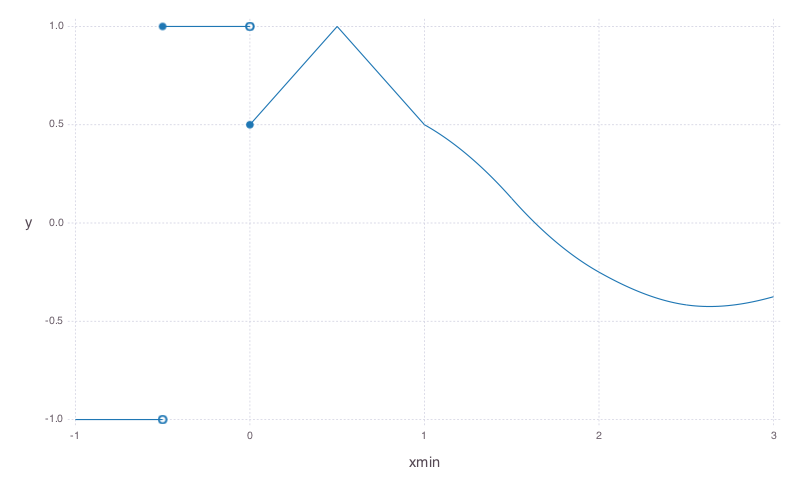
\includegraphics[width=\textwidth]{figures/piecewise-initial-function.png}
	%\caption{}
	\label{fig:not-allowed}
\end{figure}

\section{Definition}\label{definition}
